While it would be reasonable to intuitively to assume that the more information, or vector dimensions, a machine is provided during training, the more accurate it would be at classification tasks, the classic "curse of dimensionality" problem shows that this is not necessarily the case \cite{jain_1982_39} \cite{friedman_1997_on}, as overfitting, the process of fitting to noise rather than underlying patterns, \cite{overfitting} occurs when the amount of "specific information" (the dimensions of each data point's vector $\vec{L}$) is siginificantly greater than "global information" (the amount of data points in a data set) \cite{overfitting} \cite{liu_2016_overfitting}, as shown in figure \ref{fig:curse_dim}. 

\begin{figure}
    \centering
    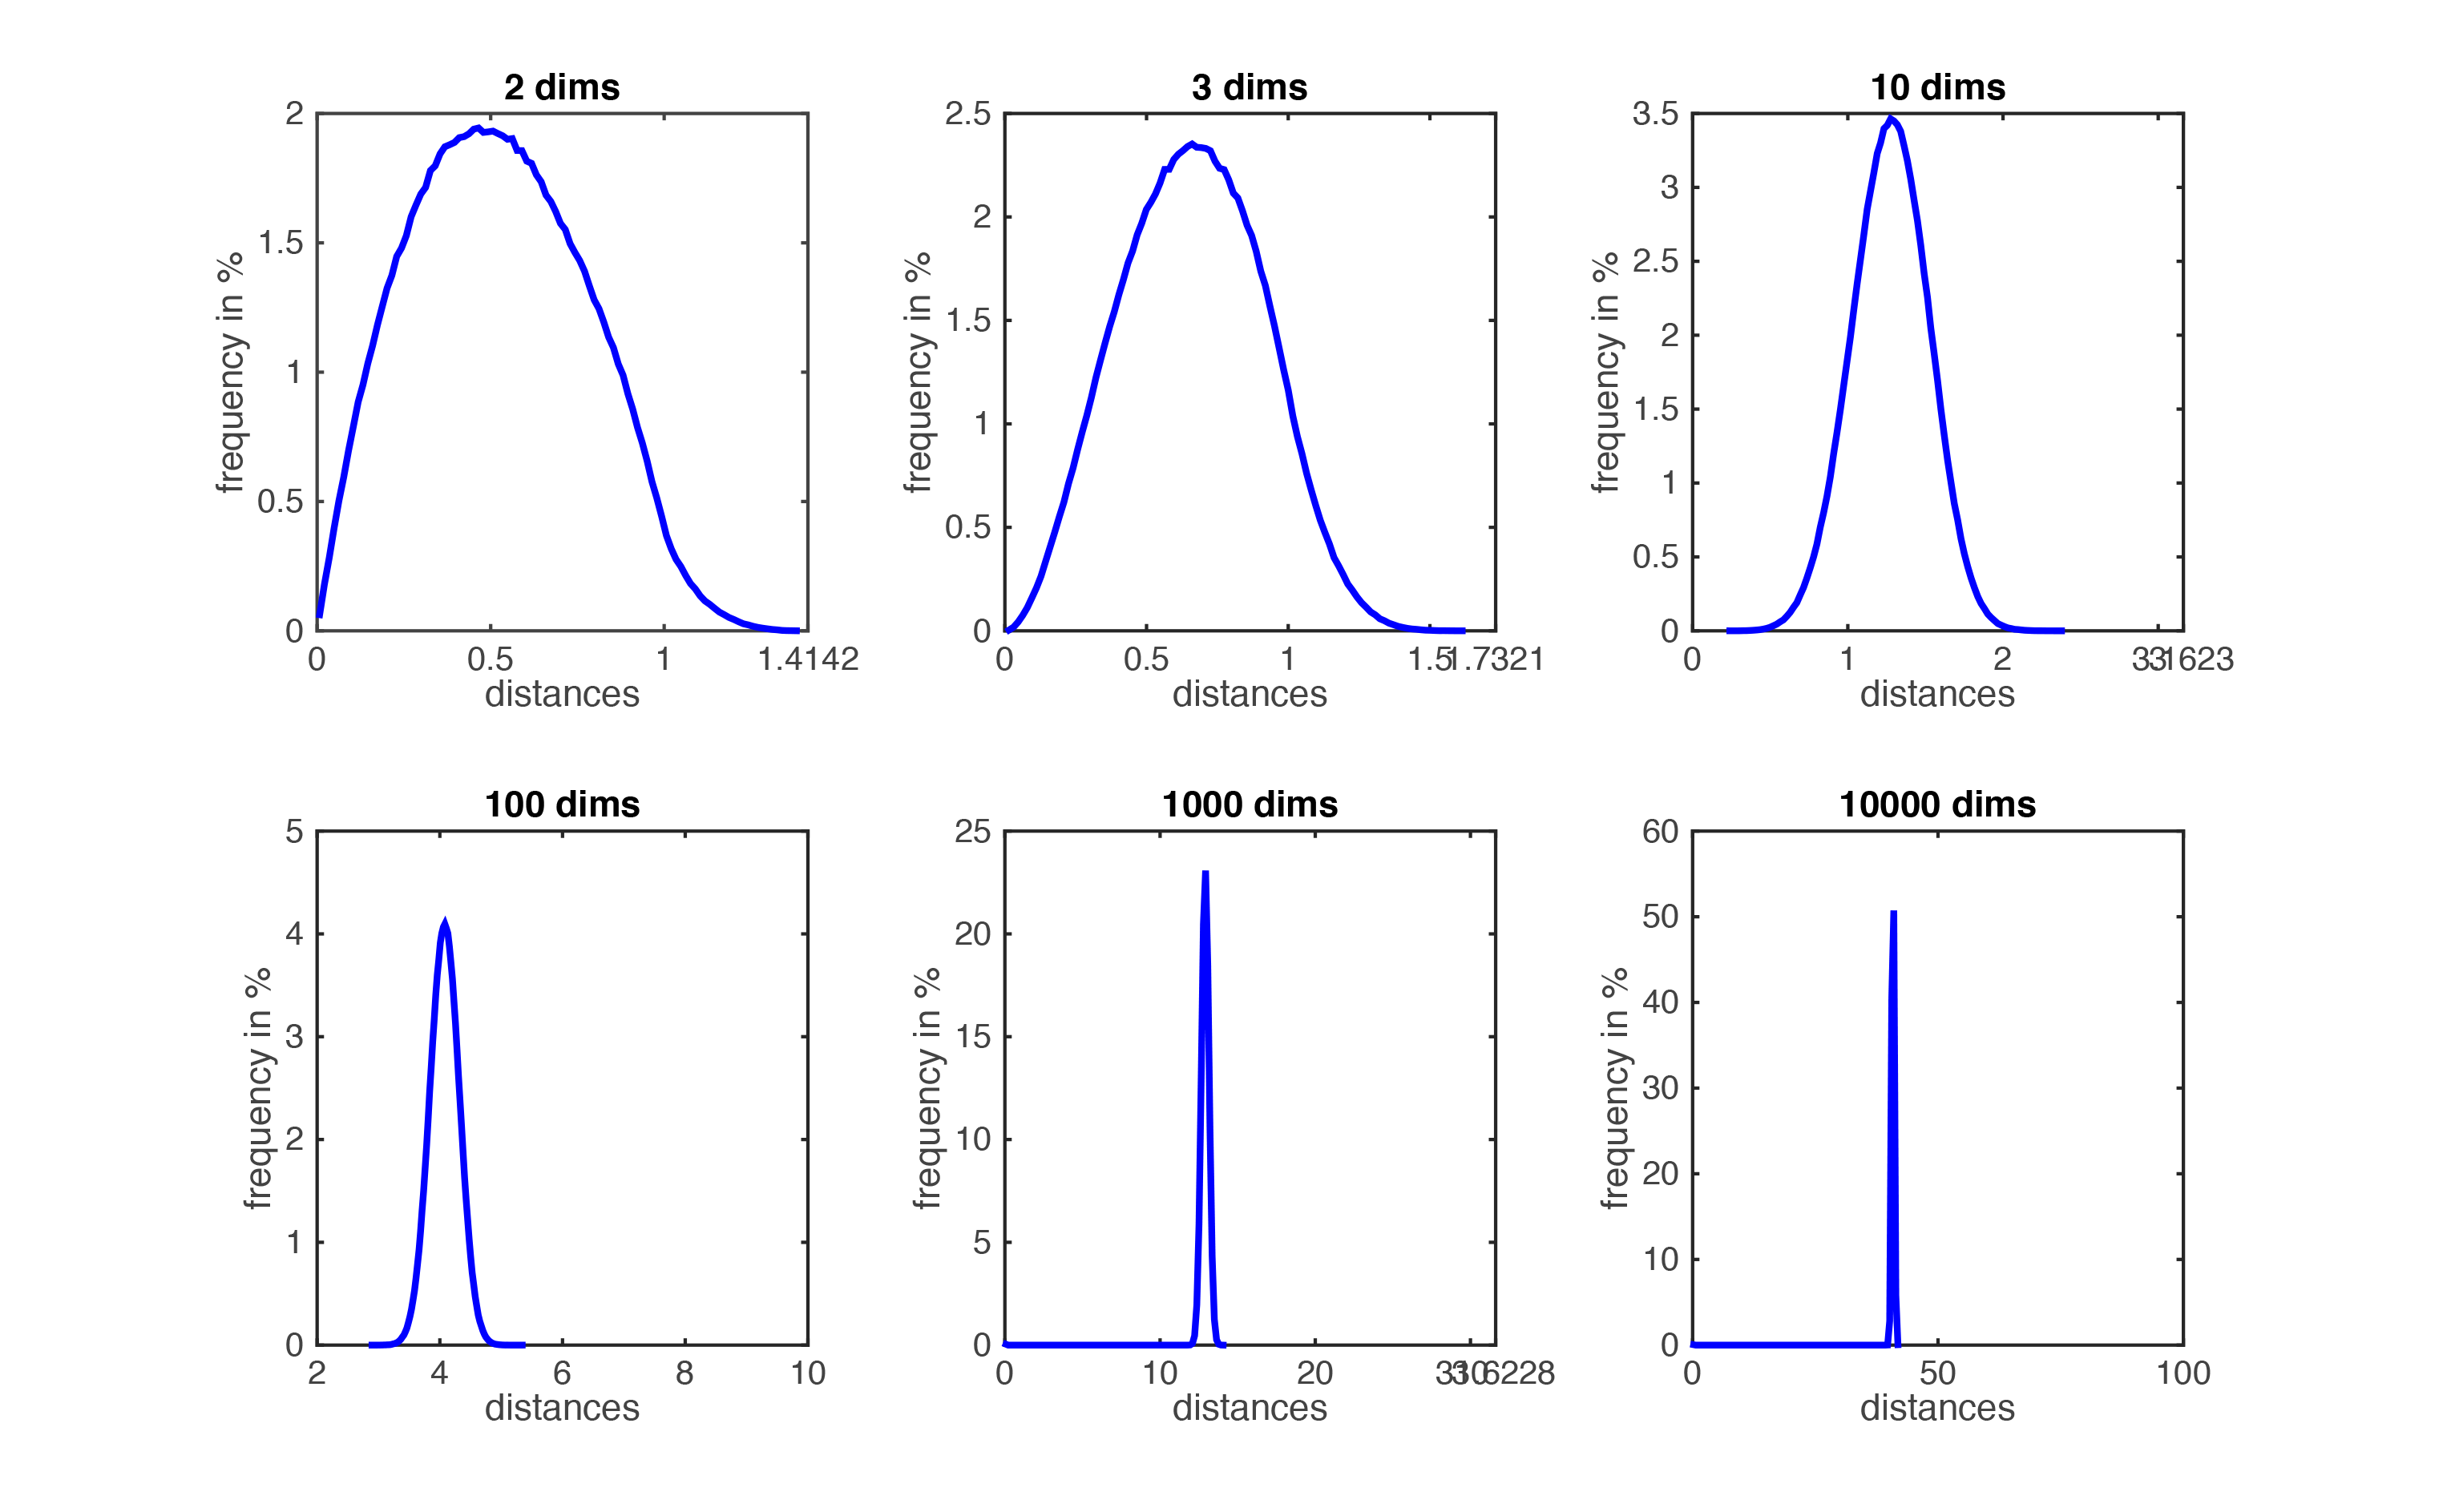
\includegraphics[width=\linewidth]{images/cursefigure.png}
    \caption{Multiple graphs which demonstrate the "curse of dimensionality". The histogram plots show the distributions of all pairwise distances between randomly distributed points within $d$-dimensional unit squares. As the number of dimensions $d$ grows, all distances concentrate within a very small range. Source: \cite{cornell_curse_notes}
}
    \label{fig:curse_dim}
\end{figure}

Jain et al. proposed a rough guideline of having at least 10 times as many training data points as input dimensions \cite{jain_2000_statistical}. Knowing that the largest possible dimensionality that can be obtained from the set of values in table \ref{table:dependent_variables} is 175392, as shown in figure \ref{}

\begin{figure}
    \centering    
    \includesvg[width=\linewidth]{images/dimension_distribution.svg}
    \caption{Kernel Density Estimation (KDE) of Dimension Values generated from various Histogram of Oriented Gradients (HOG) parameters. The blue line represents the KDE trend of the dimensions, while the red dots indicate the discrete dimension values calculated from different configurations of HOG parameters, including orientations, pixels per cell, cells per block, and block strides.}
    \label{fig:dim_distribution}
\end{figure}

\begin{table}[h]    
    \begin{minipage}{.5\linewidth}
      \renewcommand{\arraystretch}{1.5}
      \centering
        \begin{tabular}{@{} l @{\hspace{0.1cm}} l @{\hspace{0.1cm}} l @{}}    
            \toprule
            \emph{Data Set} & \emph{Positive} & \emph{Negative} \\\midrule
            INRIA Test & 361  & 543 \\ 
            Caltech Test & 2195  & 2558 \\ 
            PnPLO Test & 596  & 578 \\
            Total Training & 12794 & 14760 \\\bottomrule
        \end{tabular}
        \subcaption{Window Size (100, 50)}
    \end{minipage}%
    
    \begin{minipage}{.5\linewidth}
    \renewcommand{\arraystretch}{1.5}
      \centering
        \begin{tabular}{@{} l @{\hspace{0.1cm}} l @{\hspace{0.1cm}} l @{}}    
            \toprule
            \emph{Data Set} & \emph{Positive} & \emph{Negative} \\\midrule
            INRIA Test & 361  & 533 \\ 
            Caltech Test & 2195  & 2548 \\ 
            PnPLO Test & 596  & 475 \\
            Total Training & 12794 & 14185 \\\bottomrule
        \end{tabular}
        \subcaption{Window Size (128, 96)}
    \end{minipage}

    \vspace{0.5cm} % Space between rows of minipages

    \begin{minipage}{.5\linewidth}
    \renewcommand{\arraystretch}{1.5}
      \centering
        \begin{tabular}{@{} l @{\hspace{0.1cm}} l @{\hspace{0.1cm}} l @{}}    
            \toprule
            \emph{Data Set} & \emph{Positive} & \emph{Negative} \\\midrule
            INRIA Test & 361  & 540 \\ 
            Caltech Test & 2195  & 2554 \\ 
            PnPLO Test & 596  & 535 \\
            Total Training & 12794 & 14511 \\\bottomrule
        \end{tabular}
        \subcaption{Window Size (128, 64)}
    \end{minipage}%
    
    \begin{minipage}{.5\linewidth}
    \renewcommand{\arraystretch}{1.5}
      \centering
        \begin{tabular}{@{} l @{\hspace{0.1cm}} l @{\hspace{0.1cm}} l @{}}    
            \toprule
            \emph{Data Set} & \emph{Positive} & \emph{Negative} \\\midrule
            INRIA Test & 361  & 543 \\ 
            Caltech Test & 2195  & 2558 \\ 
            PnPLO Test & 596  & 574 \\
            Total Training & 12794 & 14731 \\\bottomrule
        \end{tabular}
        \subcaption{Window Size (112, 48)}
    \end{minipage}

\caption{Positive and Negative Sample Counts for Different Window Sizes}
\label{table:window_size_samples}
\end{table}